
\documentclass{jfm}
\usepackage{showframe}
\usepackage[english]{babel}
\usepackage{graphicx}% Include figure files
\usepackage{dcolumn}% Align table columns on decimal point
\usepackage{bm}% bold math
\usepackage[outline]{contour}
%\usepackage[mathlines]{lineno}% Enable numbering of text and display math
%\linenumbers\relax % Commence numbering lines
\usepackage[utf8]{inputenc}
\usepackage[T1]{fontenc}
\usepackage{mathptmx}
%\usepackage{patterns}
\usepackage{amsmath,amsfonts,amssymb}


\usepackage{xcolor}
\usepackage{cleveref}
\usepackage{graphicx}
\usepackage{physics}
\usepackage{tikz}
\usetikzlibrary{patterns}
\usepackage{lmodern}
\usepackage{lipsum}
\usepackage{csquotes}
\DeclareRobustCommand\full  {\tikz[baseline=-0.6ex]\draw[thick] (0,0)--(0.5,0);}
\DeclareRobustCommand\Rfull  {\tikz[baseline=-0.6ex]\draw[red,thick] (0,0)--(0.5,0);}
\DeclareRobustCommand\dotted{\tikz[baseline=-0.6ex]\draw[thick,dotted] (0,0)--(0.54,0);}
\DeclareRobustCommand\dashed{\tikz[baseline=-0.6ex]\draw[thick,dashed] (0,0)--(0.54,0);}
\DeclareRobustCommand\Rdashed{\tikz[baseline=-0.6ex]\draw[,red,thick,dashed] (0,0)--(0.54,0);}
\usepackage{adjustbox}
\usepackage{multirow}
\usepackage{subcaption}
\usepackage{MnSymbol}
\usetikzlibrary{positioning,3d}
\usetikzlibrary{graphs,automata}
\usepackage{float}
\usepackage{pgfplots}
\usepgfplotslibrary{fillbetween}



\pgfplotsset{compat=1.15
 ,colormap={parula}{
rgb255=(53,42,135)
rgb255=(15,92,221)
rgb255=(18,125,216)
rgb255=(7,156,207)
rgb255=(21,177,180)
rgb255=(89,189,140)
rgb255=(165,190,107)
rgb255=(225,185,82)
rgb255=(252,206,46)
rgb255=(249,251,14)
        }}
        \shorttitle{ML report}
\shortauthor{J.Yang}
    \title{ML report}
% Force line breaks with \\

\author{Jiasheng Yang\aff{1}\corresp{\email{jiasheng.yang@kit.edu}}}

\affiliation{\aff{1}Institute of Fluid Mechanics, Karlsruhe Institute of Technology, Karlsruhe, Germany}

\begin{document}

\section{Simulation setup}
Turbulent channel with constant pressure gradient (CPG).
$Re_\tau=u_\tau(H-k_{md})/\nu$, where $u_tau=\sqrt{\tau_w/rho}$ and $\tau_w=-P_x(H-k_{md})$.
\begin{figure}
\centering
   % 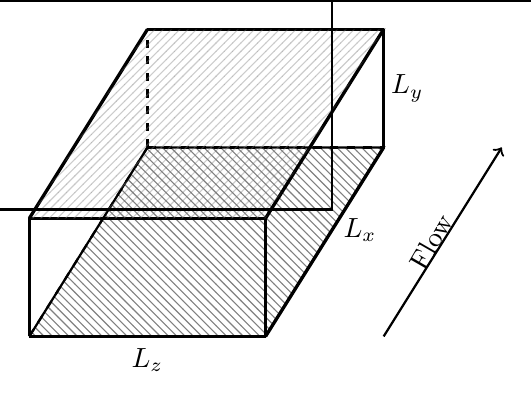
\begin{tikzpicture}[thick,scale=3]
    \coordinate (A1) at (0, 0);
    \coordinate (A2) at (0, 0.5);
    \coordinate (A3) at (1, 0.5);
    \coordinate (A4) at (1, 0);
    \coordinate (B1) at (0.5, 0.8);
    \coordinate (B2) at (0.5, 1.3);
    \coordinate (B3) at (1.5, 1.3);
    \coordinate (B4) at (1.5, 0.8);
    \draw[pattern=north west lines, pattern color=gray] (A1) -- (B1) -- (B4) -- (A4);
    \coordinate (AR1) at (1.5, 0);
    \coordinate (AR2) at (2, 0.8);

    \draw[very thick] (A1) -- (A2);
    \draw[very thick] (A2) -- (A3);
    \draw[very thick] (A3) -- (A4);
    \draw[very thick] (A4) -- (A1);

    \draw[dashed] (A1) -- (B1);
    \draw[dashed] (B1) -- (B2);
    \draw[very thick] (A2) -- (B2);
    \draw[very thick] (B2) -- (B3);
    \draw[very thick] (A3) -- (B3);
    \draw[very thick] (A4) -- (B4);
    \draw[very thick] (B4) -- (B3);
    \draw[dashed] (B1) -- (B4);
    \draw[->] (AR1) -- (AR2);

    %\draw[fill=black!20,opacity=0.5] (A1) -- (A2) -- (A3) -- (A4);
    %\draw[fill=red,opacity=0.6] (A1) -- (A2) -- (B2) -- (B1);
    %\draw[fill=black,opacity=0.6] (B1) -- (B2) -- (B3) -- (B4);
    %\draw[fill=blue,opacity=0.6] (A3) -- (B3) -- (B4) -- (A4);
    \draw[pattern=north east lines, pattern color=gray, opacity=0.4] (A2) -- (B2) -- (B3) -- (A3);
    \node[] at (0.5,-0.10) {$L_z$};
    \node[] at (1.4,0.45) {$L_x$};
    \node[] at (1.6,1.05) {$L_y$};
    \node[rotate=60] at (1.7,0.4) {Flow};
\end{tikzpicture}
   \includegraphics[width=10cm]{Figures/Domain.png}
    \caption{Schematic representation of simulation domain with an example pseudo-realistic surface mounted. Normalization of lengths with $H$ is applied in the figure.}
    \label{fig:domain}
\end{figure}
\begin{table}
    \centering
    \begin{tabular}{ccccccccc}
         SurfaceID&$Re_\tau$&$L_x/H$&$L_z/H$&$N_x$&$N_z$&$\Delta_x^+$&$\Delta_z^+$&$\Delta_{y,k}^+$\\[3pt]
         0-199&500&2.4&0.8&480&160&2.5&2.5&$\approx1.74$\\
         200-399&500&3&1&576&192&2.6&2.6&$\approx1.74$
    \end{tabular}
    \caption{Simulation domain setup}
\end{table}
\section{Roughness configuration}
\label{Roughness}
Identical $Re_\tau$, variying $k_99$
\begin{figure}
\includegraphics[width=0.6\linewidth]{Figures/Pairplot.png}
\end{figure}
\subsection{PDF}
Weibull:$$f(k)= \lambda \beta^\lambda k^{(\lambda-1)}e^{-(\beta k)^\lambda},$$ 
Bimodal:$$k(i)=min\{\Phi_{0,1}(i),\Phi_{-\lambda,\lambda}(i)\},$$
Gaussian:$$f(i)=\frac{1}{\sigma\sqrt{2\pi}}e^{-\frac{1}{2}(\frac{i-\mu}{\sigma})^2}$$
\subsection{PS}
$\lambda_0=0.8H$ (1-199), $=1H$ (200-399).
$\lambda_1=0.04H$.
PS normalized by $\lambda_{diff}=\lambda_0-\lambda_1$.
Roll-off length: $L_r/\lambda_{diff}=\Phi_{0.4,0.04}$.
PS slope:$\theta_p=-|\Phi_{0.75,0.3}|$.
Randomize along PS(20): PS$(i)-\Phi_{0,0.5*i}$.
\begin{figure}
        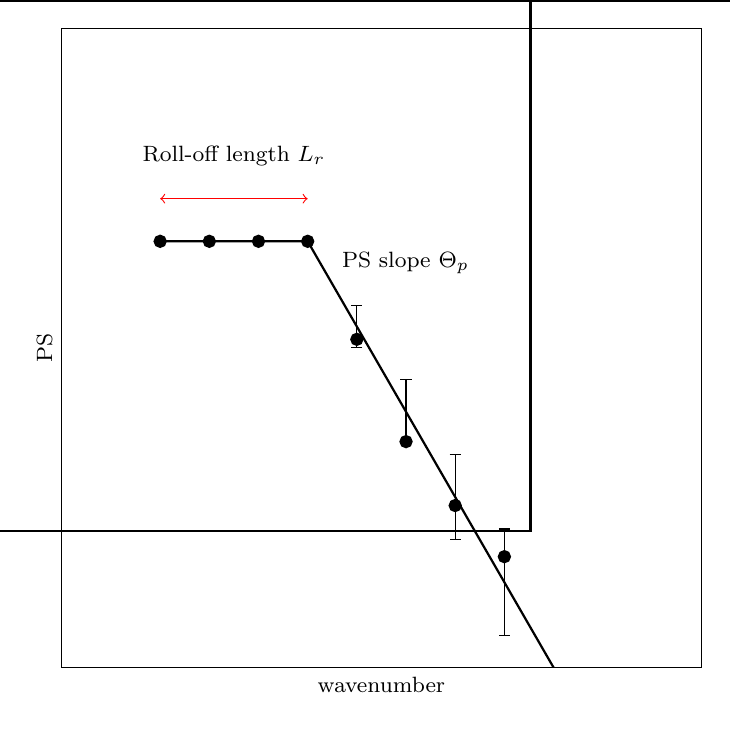
\begin{tikzpicture}[]
        \centering
        \begin{axis}[
            ylabel={PS},
            xlabel={wavenumber},
            ymin=0, ymax=1.5,
			xmax=1.3,
			xmin=0,
			xtick=\empty,
			ytick=\empty,
            width=.8\textwidth,
            height=.8\textwidth,
            label style={font=\footnotesize},
            legend style={font=\tiny,anchor=south east},
                        legend pos=south east,
            tick label style={font=\footnotesize}
            ]

			\addplot [
            black,thick,no marks,
            ]
            coordinates{
            (0.2, 1)
            (0.5, 1)
            (1,0)
            };
			\draw[<->,red] (0.2,1.1) -- (0.5,1.1);
			\node[] at (0.35,1.2) {\footnotesize{Roll-off length $L_r$}};
			\node[right] at (0.55,0.95) {\footnotesize{PS slope $\Theta_p$}};
			\addplot [
            black,thick,only marks,mark=*,
            ]
            coordinates{
            (0.2, 1)
            (0.3, 1)
			(0.4, 1)
			(0.5, 1)
			(0.6,0.77)
			(0.7,0.53)
			(0.8,0.38)
			(0.9,0.26)
            };
									\addplot[
        only marks,
        mark=X,
        black,
        error bars/.cd, y dir=both, y explicit,
    ] plot coordinates {
                    (0.6, 0.8)+=(0,0.05) -=(0,0.05)
    };
										\addplot[
        only marks,
        mark=X,
        black,
        error bars/.cd, y dir=both, y explicit,
    ] plot coordinates {
                    (0.7, 0.6)+=(0,0.075) -=(0,0.075)
					    };
							\addplot[
        only marks,
        mark=X,
        black,
        error bars/.cd, y dir=both, y explicit,
    ] plot coordinates {
                    (0.8, 0.4)+=(0,0.1) -=(0,0.1)
					    };
							\addplot[
        only marks,
        mark=X,
        black,
        error bars/.cd, y dir=both, y explicit,
    ] plot coordinates {
                    (0.9, 0.2)+=(0,0.125) -=(0,0.125)
					    };
        \end{axis}
        \end{tikzpicture}
\caption{PS Sketch}
\end{figure}
\end{document}
%
% ****** End of file aipsamp.tex ******